
\chapter{Single cells analysis}
\label{chap:UnitsAnalysis}
In this chapter I present the analysis performed on single cells, before to apply the cell-assembly algorithm to the data set.
The principal interest of the project was to investigate the nature of Ventral Striatum and Ventral Tegmental Area. Furthermore it is well known that in both regions different units types are present, a schematic illustration of the brain-circuit of interest is shown in figure(\ref{fig:Brain}).
\begin{figure}
    \centering
    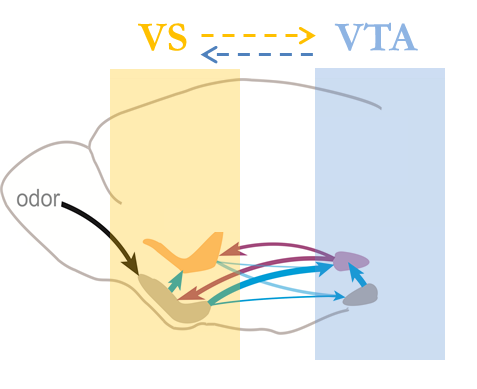
\includegraphics[width=0.45\textwidth]{BrainVSVTA.png}
    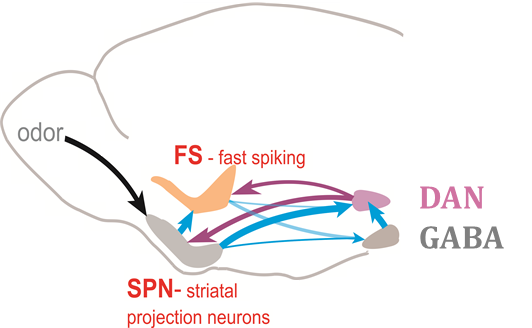
\includegraphics[width=0.45\textwidth]{Brain.png}
    \caption{Caption}
    \label{fig:Brain}
\end{figure}
The circuit effect of interactions makes the nature of themselves puzzling, to figure out which interactions are specifically involved in Reward Prediction and Reward Prediction error, it was matter of interest to understand whether inter-regional interactions between specific cell types have specific characteristics, not found in other cell types.
The data-set included $803$ VS units and $272$ VTA units in total, that were classified in sub-types, specifically VS units were classified as either striatal projection neurons (SPNs), fast-spiking neurons (FSNs) or cholinergic interneurons(CINs), according to their firing pattern characteristics computed using only spikes during the inter-trials interval and after session. Units with a firing rate higher than $12 Hz$ were assigned as FSNs and all units with a firing rate below $2 Hz$ as SPNs. Units in the remaining range were designed as putative regular-firing  CINs if the CV or their $ISI$ distribution was less than $1.2$ and ISIs less than $60 ms$ contributed no more than $20\%$ of all ISIs. Finally the resting units were characterized as SPNs or FSNs if they ever were silent for more than $2 s$. Using this classification mean normalized autocorrelations and mean waveforms have canonical patterns. It is important to make a clarification about FSN: it can be assumed that the recorded FSNs are pallidal neurons, in fact FSNs in Striatum represent only $<5\%$ of the population({\color{red}ask for a paper to cite}), while pallidal units have higher firing rate ({\color{red} sk for a paper to cite}). %(\ref{fig:AutoVS}).
VTA units were instead classified as dopaminergic neurons (DAN), gabaergic units (GABA), and glutamatergic neurons (GLU) according to their task related activity using a clustering approach adapted from (\cite{Uchida}). First, response were characterized for the relevant time spans ({\color{red}ask Max for the updated intervals}(CS+ from 0 to 0.5 and US from -0.5 to 0 and from 0 to 0.5), significant task related response were assessed with Friedman test, and only significant units ($p<0.05$) were included in the clustering classification.{\color{red}part of classification has to be included}

\begin{figure}
  \centering
    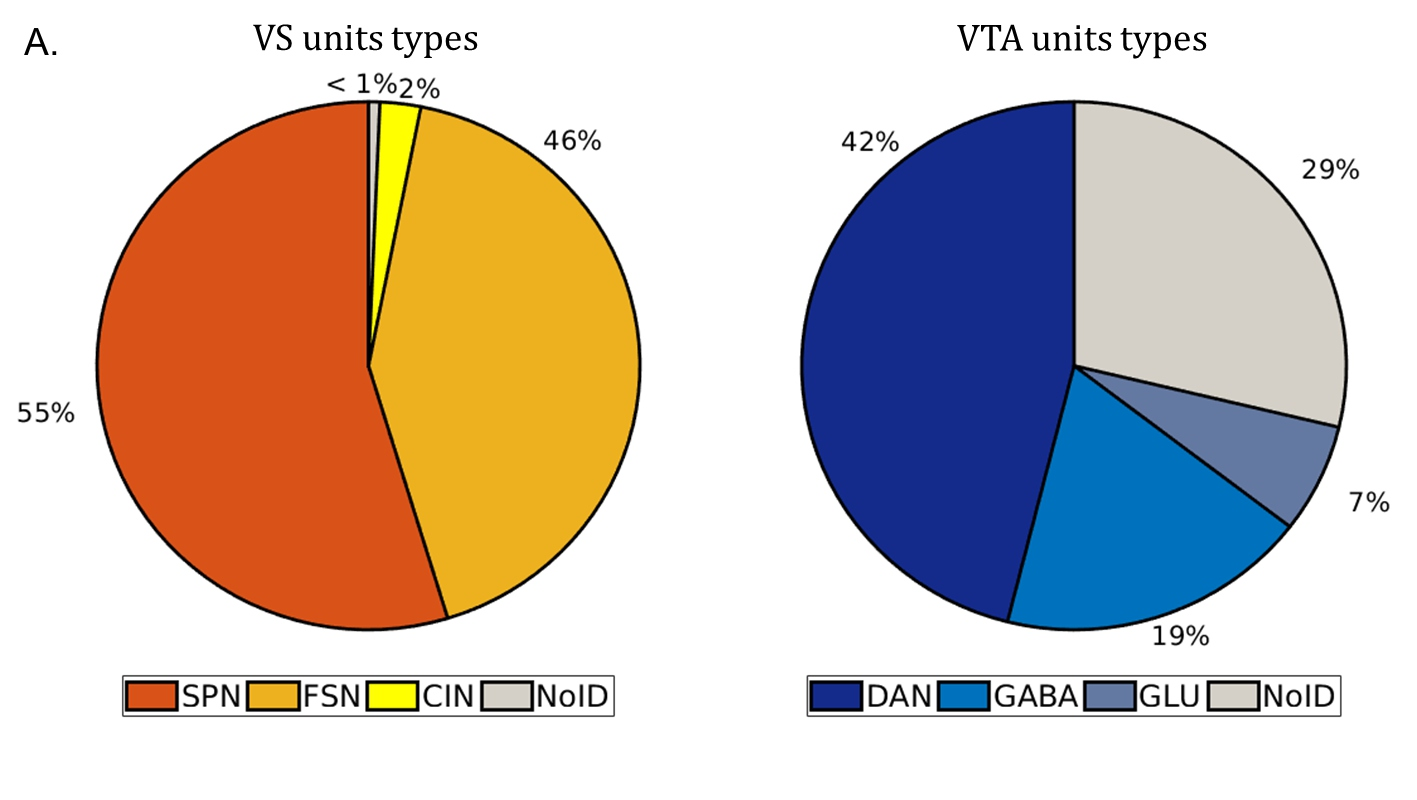
\includegraphics[scale=0.5]{figures/PieRegions1.pdf}
   \caption{Left: units types pie chart in Ventral Striatum. Right: units types pie chart in Ventral Tegmental Area}
    \label{fig:PieRegions}
\end{figure}

\begin{figure}
  \centering
    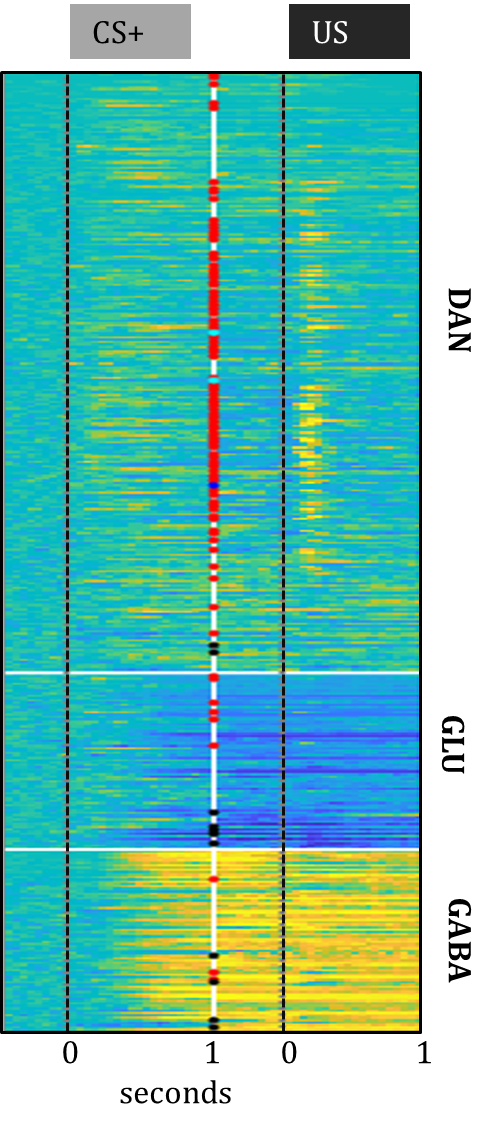
\includegraphics[scale=0.75]{figures/ClassificationUnits.png}
   \caption{VTA classification according to units task related activity using a clustering approach adapted from (\cite{Uchida}). In this study we focused on dopaminergic and gabaergic units in assemblies. Dopaminergic units show a phasic response to the reward, whereas gabaergic units are tonically active neurons.}
    \label{fig:ClassificatonVTA}
\end{figure}
%\begin{figure}
 %   \centering
  %  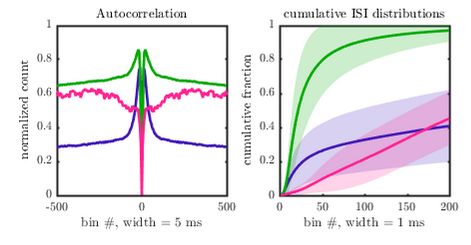
\includegraphics[scale=0.7]{figures/AutocorrelationVSunits.png}
   % \caption{Caption}
    %\label{fig:AutoVS}
%\end{figure}({\color{red}citation of graybiel 2005 if it is the rigth paper})
%distributed as shown in fig.(\ref{fig:GlobalPie})
